A Vertical Scrolling Rhythm Game (VSRG) is simply a rhythm game where notes travel from top-to-bottom or bottom-to-top to hit a receptor.
The timing when it hits a receptor is usually related to an instrument in the music, thus the player mimics the play of the actual instrument.
There are several ways to input, either using a keyboard, a pressure-sensitive device, a custom controller, and many more.
To limit our scope, we will only consider keyboard inputs, one of the most popular way to play this genre.

\begin{figure}[H]
    \centering
    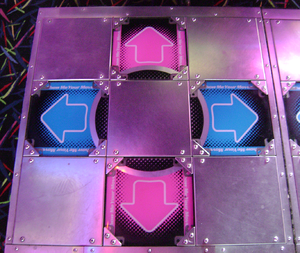
\includegraphics[scale=0.5]{imgs/300px-Dance_Dance_Revolution_Extreme_arcade_machine_left_side_stage}
    \caption{Pressure Sensitive Dance Dance Revolution device to be played with feet.}
    \label{fig:ddr_pressure}
\end{figure}

\begin{figure}[H]
    \centering
    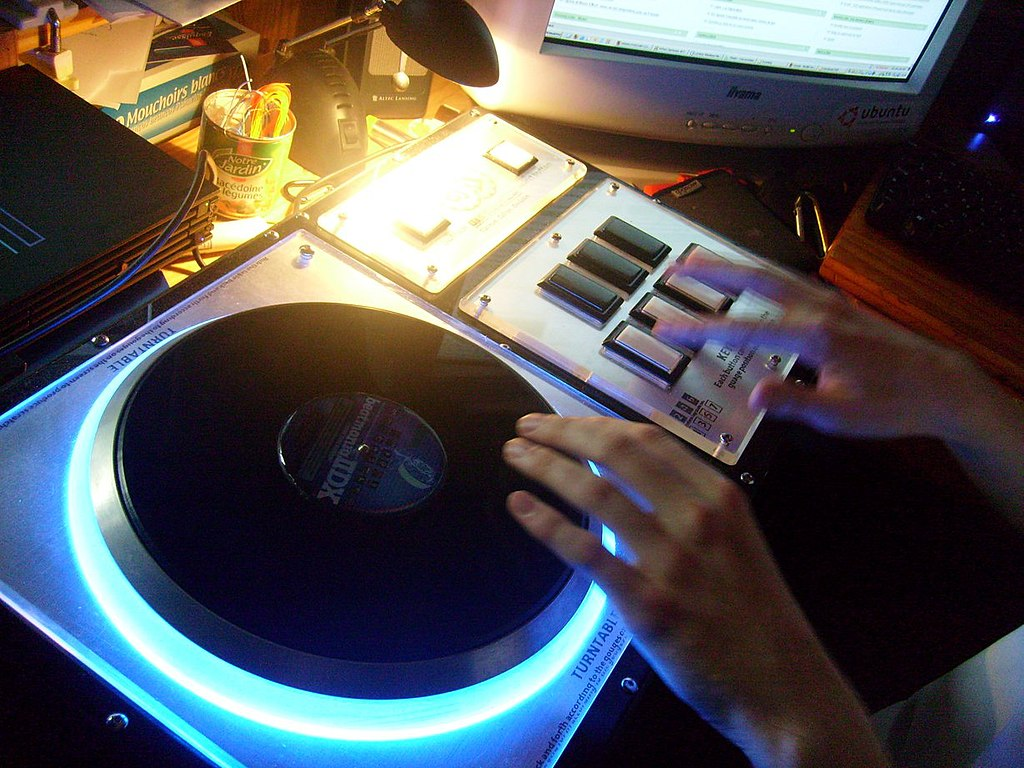
\includegraphics[scale=0.3]{imgs/1024px-Beatmania_IIDX_DAOPEE_Controller}
    \caption{Beatmania IIDX Controller to be played with hands.}
    \label{fig:iidx_controller}
\end{figure}

\begin{figure}[H]
    \centering
    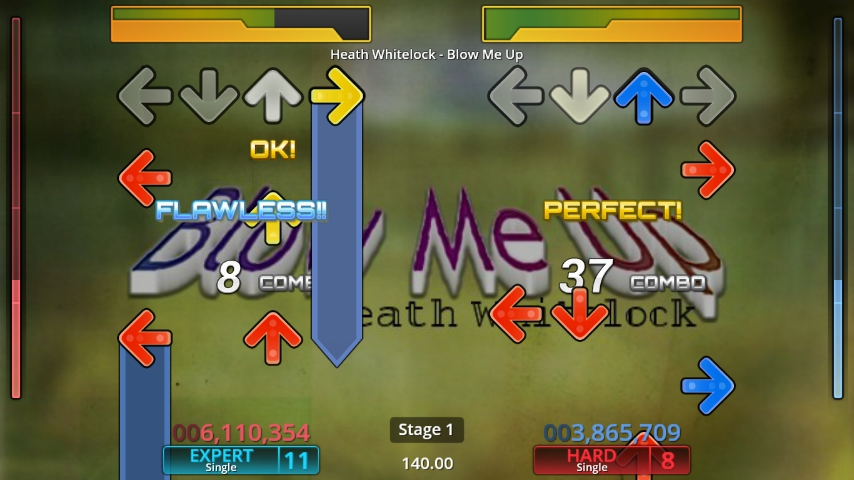
\includegraphics[scale=0.3]{imgs/StepMania_5.0.5_Demo}
    \caption{Image of StepMania 5.0.5. Shows gray arrow receptors on top, and red, yellow, blue notes travelling upwards towards the receptor.}
    \label{fig:stepmania}
\end{figure}

To illustrate the gameplay, I show StepMania in Figure~\ref{fig:stepmania}, one of the more popular old VSRGs.
We can observe the notes in red, blue, yellow, indicative of their rhythm, travelling upwards to reach the
receptor in gray.
Upon reaching it, the player is prompted to input correspondingly, where they will be
judged on their rhythmic precision.

One of the major pitfalls of rhythm games such as this, is difficulty estimation.
Due to its complexity, creators usually resort to manual annotation.
Alternatively, most popularly, difficulty is estimated by note density, for it has high correlation to difficulty.
This method, however, neglects the order of the notes, note patterns, thus leading to many anomalous density-estimated maps.

\begin{figure}[H]
    \centering
    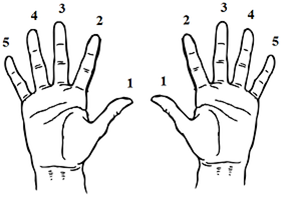
\includegraphics{imgs/finger-notation}
    \caption{Annotated Finger positions}
    \label{fig:finger_notation}
\end{figure}